%--------------------------------------------------------------------------------------------------
\section{Content of the AMIDST software} \label{sec:Content}
%--------------------------------------------------------------------------------------------------

The AMIDST software is an open source Java project based on Maven automation tool. Maven ensures a description of how the software project is built and its dependencies on other external modules, Java libraries, and plug-ins.  

The AMIDST software consists of:

\begin{itemize}

\item A README file containing a short description of the content of the toolbox, and information on how to compile and run the command line application.

\item The script \texttt{compile.sh} that compiles the whole AMIDST project and create a \texttt{.jar} file in the ./target folder.

\item The script \texttt{run.sh} that should be used to run some classes. For instance, \texttt{./run.sh} \texttt{eu.amidst.examples.DynamicNaiveBayesClassifierDemo} runs a demo for learning a dynamic naive Bayes classifier.

\item The source code organised in packages, as shown in Figure \ref{Figure:SoftwareContent}, and consisting of the implementation of the data structures, the database functionalities, the AMIDST models, and the different considered algorithms for learning and inference. 

\end{itemize}


\begin{figure}[ht!]
\begin{center}
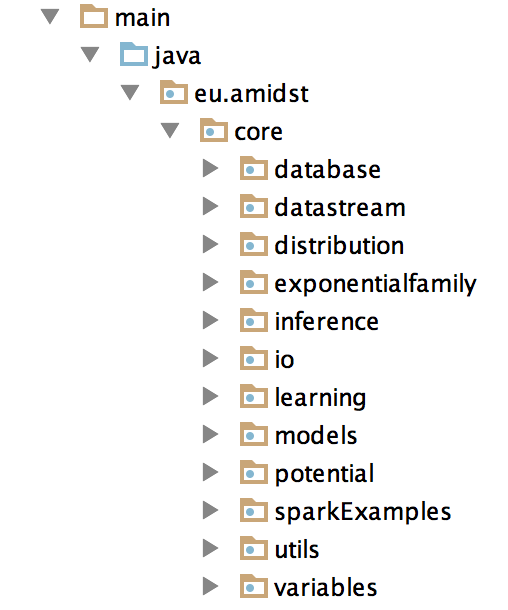
\includegraphics[scale=0.75]{./figures/SoftwareContent}
\caption{\label{Figure:SoftwareContent}Content of the AMIDST software.}
\end{center}
\end{figure}